\subsection{Project Management Essentials}

\subsubsection{Project}

\noindent\textbf{Project}: A temporary endeavor undertaken to create a unique product, service, or result.

\noindent\textbf{Key characteristics}:

\begin{itemize}
    \item \textbf{Temporary}: Has a defined start and end date.
    \item \textbf{Unique}: Outcome is not routine, even if processes are repeatable.
    \item \textbf{Progressive elaboration}: Develops in steps and continues by increments.
\end{itemize}

\subsubsection{Success criteria}

\begin{itemize}
    \item \textbf{On-Time Delivery}: Meets the agreed schedule.
    \item \textbf{On-Budget}: Stays within allocated costs.
    \item \textbf{Meets Scope \& Quality}: Delivers all required features with acceptable quality standards.
    \item \textbf{Stakeholder Satisfaction}: End users, clients, and management are satisfied with the result.
    \item \textbf{Business Value}: Delivers measurable benefits such as cost savings, efficiency gains, or competitive advantage.
\end{itemize}

\subsubsection{Fail Reasons}

\begin{itemize}
    \item \textbf{Poor Scope Definition}: Unclear requirements, frequent changes.
    \item \textbf{Unrealistic Timelines or Budgets}: Overly optimistic estimates.
    \item \textbf{Weak Stakeholder Engagement}: Lack of buy-in from sponsors or end users.
    \item \textbf{Inadequate Risk Management}: Failing to anticipate and mitigate issues.
    \item \textbf{Poor Communication}: Misalignment between teams and stakeholders.
    \item \textbf{Resource Issues}: Lack of skilled staff or technology limitations.
\end{itemize}

\subsection{Project Management Methodologies}

\noindent\textbf{Project management methodology}: A structured approach that guides how a project is planned, executed, and delivered.

\noindent\textbf{Main purpose} of following a methodology:

\begin{itemize}
    \item Provides a framework to organise work
    \item Improves efficiency and communication
    \item Helps manage risks and deliver consistent results
\end{itemize}

\subsubsection{Waterfall Methodology}

\begin{figure}[h]
    \centering
    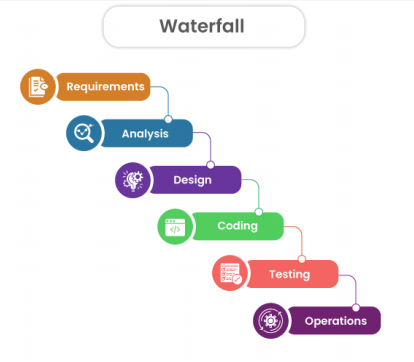
\includegraphics[width=0.5\linewidth]{figures/Week 3/Waterfall.png}
\end{figure}

Sequential, linear approach where each phase must be completed before the next begins.

\bigskip

\textbf{Benefits:}

\begin{itemize}
    \item Clear structure and documentation.
    \item Easy to manage with well-defined deliverables.
    \item Works well when requirements are stable.
\end{itemize}

When to use: Projects with fixed scope and minimal expected changes (e.g., compliance software, construction projects).

\bigskip

\textbf{Disadvantages:}

\begin{itemize}
    \item \textbf{Inflexibility to Changes}: Once a phase is completed, it’s difficult and costly to go back and make changes without affecting the entire project.
    \item \textbf{High Risk for Long Projects}: In lengthy projects, technology, user expectations, or market conditions might change before delivery, making the end product outdated.
    \item \textbf{Over-reliance on Initial Documentation}: The success of the project heavily depends on the accuracy and completeness of initial requirements and documentation.
    \item \textbf{Limited Stakeholder Engagement During Development} Once requirements are set, stakeholders are less involved until final delivery, which can lead to misalignment with expectations.
\end{itemize}

\subsubsection{Agile Methodology}

\begin{figure}[h]
    \centering
    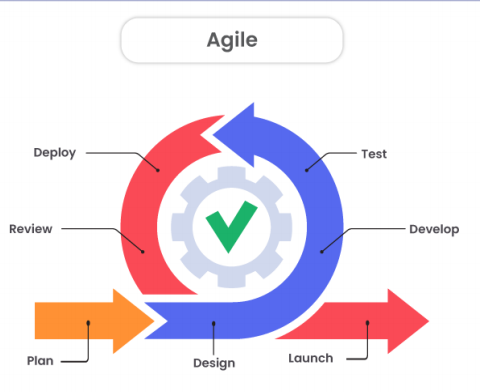
\includegraphics[width=0.5\linewidth]{figures/Week 3/Agile.png}
\end{figure}

Iterative, flexible approach focusing on delivering small, incremental improvements. Uses short work cycles called \textbf{sprints}.

\bigskip

\textbf{Benefits:}

\begin{itemize}
    \item Adapts to changing requirements.
    \item Encourages stakeholder feedback early and often.
    \item Delivers working software faster.
\end{itemize}

When to use: Projects where requirements are evolving (e.g., mobile apps, SaaS products)

\subsubsection{DevOps Approach}

\begin{figure}[h]
    \centering
    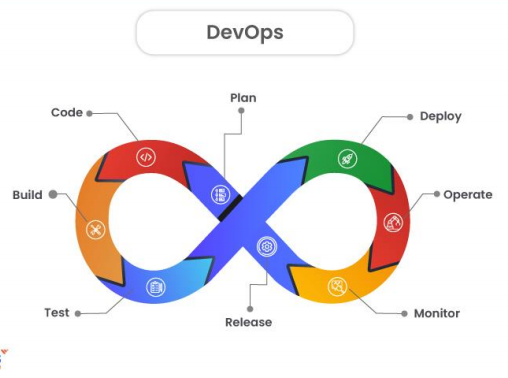
\includegraphics[width=0.5\linewidth]{figures/Week 3/DevOps.png}
\end{figure}

Combines software development (Dev) and IT operations (Ops) for continuous integration, delivery, and monitoring. Focuses on automation, collaboration, and rapid releases.

\bigskip

\textbf{Benefits:}

\begin{itemize}
    \item Faster release cycles.
    \item Improved software quality through continuous testing and integration.
    \item Enhanced collaboration between dev and ops teams.
\end{itemize}

When to use: Cloud-based applications, high frequency release environments, or products requiring rapid deployment and scaling.

\subsubsection{Waterfall VS Agile VS DevOps}

\begin{table}[h]
\centering
\begin{tabular}{|c|c|c|cl|}
\hline
\textbf{Feature}                                                           & \textbf{Waterfall}   & \textbf{Agile}        & \multicolumn{2}{c|}{\textbf{DevOps}}               \\ \hline
\textbf{Approach}                                                          & Sequential           & Iterative             & \multicolumn{2}{c|}{Continuous}                    \\ \hline
\textbf{Flexibility}                                                       & Low                  & High                  & \multicolumn{2}{c|}{High}                          \\ \hline
\textbf{Delivery}                                                          & End of project       & Incremental           & \multicolumn{2}{c|}{Continuous}                    \\ \hline
\textbf{\begin{tabular}[c]{@{}c@{}}Stakeholder\\ Involvement\end{tabular}} & Low                  & High                  & \multicolumn{2}{c|}{High}                          \\ \hline
\textbf{Best for}                                                          & Fixed scope projects & Evolving requirements & \multicolumn{2}{c|}{Rapid deployment environments} \\ \hline
\textbf{Speed}                                                             & Slower               & Faster                & \multicolumn{2}{c|}{Fastest}                       \\ \hline
\end{tabular}
\end{table}

\subsection{Rise of the continuous IT Lifecycle}

\subsubsection{Business and IT Silos}

\indent

In traditional development, the development team and operations team worked in silos.

Development teams focused on functionality, features, and non-functional requirements.

Operations teams focused on cost, reliability, security, risk, and manageability.

\subsubsection{Traditional Linear Approach}

\begin{figure}
    \centering
    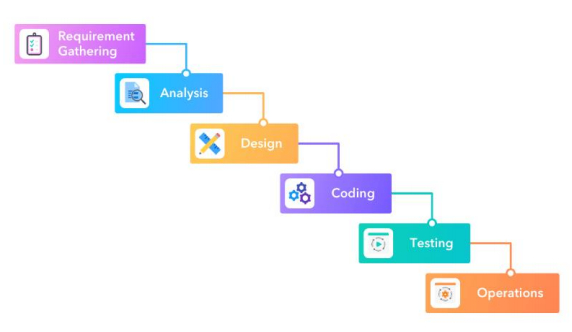
\includegraphics[width=0.5\linewidth]{figures/Week 3/Linear Approach.png}
\end{figure}

Traditionally, the approach to managing the lifecycle of a software application was a set of linear, sequential, stages that managed the development of the application as a project.

The waterfall method was typically used for this project management and was an earlier foundation of the PMBOK (Project Management body of Knowledge), and SDLC (Software Development Life Cycle) methodologies.

\subsubsection{Shift from Linear to Continuous}

\begin{table}[h]
\centering
\begin{tabular}{|c|c|}
\hline
\textbf{The Old model (Linear)}                                                                                     & \textbf{The New model (Continuous)}                                        \\ \hline
\begin{tabular}[c]{@{}c@{}}One way flow\\ Plan \textgreater Build \textgreater Deploy \textgreater End\end{tabular} & \begin{tabular}[c]{@{}c@{}}Ongoing\\ incremental improvements\end{tabular} \\ \hline
Large, infrequent releases.                                                                                         & Frequent, small releases                                                   \\ \hline
\end{tabular}
\end{table}

\noindent\textbf{Why the change?}

\begin{itemize}
    \item Need for agility in a fast-moving digital environment.
    \item Rising customer expectations for quick fixes and new features.
\end{itemize}

\bigskip

\noindent\textbf{Factors driving this shift}:

\begin{itemize}
    \item \textbf{Digital Transformation}: Need to keep pace with competitors.
    \item \textbf{Customer Expectations}: Users expect quick updates and fixes.
    \item \textbf{Cloud \& Automation}: Enables faster, safer deployments.
    \item \textbf{Agile \& DevOps Practices}: Promote collaboration and speed.
    \item \textbf{Data-Driven Decisions}: Continuous monitoring informs priorities.
\end{itemize}

\subsubsection{Continuous IT Lifecycle}

\begin{figure}[h]
    \centering
    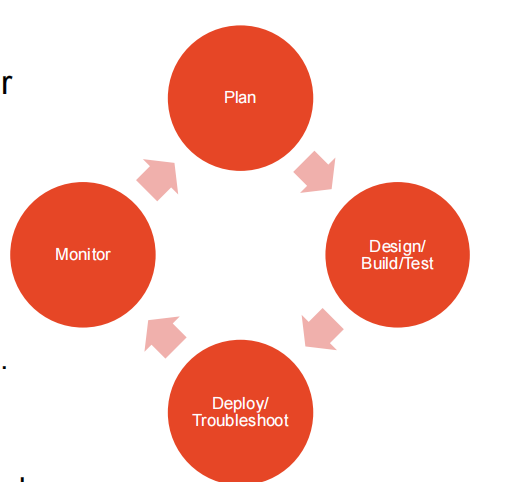
\includegraphics[width=0.5\linewidth]{figures/Week 3/Continuous IT Lifecycle.png}
\end{figure}

\noindent\textbf{Continuous IT Lifecycle}: A recurring, iterative approach to managing IT systems where improvement and delivery never stop. Instead of ending after deployment, IT work continues with \textbf{monitoring, feedback, and updates}. Enables faster innovation and responsiveness.

\bigskip

\noindent\textbf{Elements of the Continuous IT Lifecycle}:

\begin{itemize}
    \item Planning the development aligned with business strategy.
    \item Establishing the requirements, designing, building (or acquiring), testing.
    \item Deploying to the live environment (integrating with other e.g. other applications, middleware, operating systems), maintaining service levels (e.g. troubleshooting) and measuring performance
    \item Monitoring the value to the organisation. Depending on the results of the monitoring a new planning process would begin for refinements and improvements, making the cycle continuous (that cycle time can vary from very short to long)
\end{itemize}

\subsubsection{Linear Approach VS Continuous Approach}

\begin{table}[h]
\centering
\begin{tabular}{|c|c|l|}
\hline
\textbf{Aspect}                           & \textbf{Approach}                                                       &                                                                                                                                        \\ \hline
\multirow{2}{*}{\textbf{Definition}}      & \textbf{Linear}                                                         & \begin{tabular}[c]{@{}l@{}}A step-by-step,sequential method where each phase is\\ completed before moving to the next.\end{tabular}    \\ \cline{2-3} 
                                          & \textbf{\begin{tabular}[c]{@{}c@{}}Continuous\\ Lifecycle\end{tabular}} & \begin{tabular}[c]{@{}l@{}}A flexible,iterative approach where development,\\ testing,and deployment happen continuously.\end{tabular} \\ \hline
\multirow{2}{*}{\textbf{Process Flow}}    & \textbf{Linear}                                                         & \begin{tabular}[c]{@{}l@{}}One-way,structured progression\\ (e.g., Waterfall model).\end{tabular}                                      \\ \cline{2-3} 
                                          & \textbf{\begin{tabular}[c]{@{}c@{}}Continuous\\ Lifecycle\end{tabular}} & \begin{tabular}[c]{@{}l@{}}Cyclical and iterative,allowing feedback and\\ improvements(e.g., Agile, DevOps).\end{tabular}              \\ \hline
\multirow{2}{*}{\textbf{Flexibility}}     & \textbf{Linear}                                                         & \begin{tabular}[c]{@{}l@{}}Rigid-Changes are difficult to implement \\ once a phase is completed.\end{tabular}                         \\ \cline{2-3} 
                                          & \textbf{\begin{tabular}[c]{@{}c@{}}Continuous\\ Lifecycle\end{tabular}} & \begin{tabular}[c]{@{}l@{}}Highly adaptable-Continuous improvements \\ and iterations are possible.\end{tabular}                       \\ \hline
\multirow{2}{*}{\textbf{Risk Management}} & \textbf{Linear}                                                         & \begin{tabular}[c]{@{}l@{}}High risk-Issues are often detected\\ late in the process(e.g.,during testing).\end{tabular}                \\ \cline{2-3} 
                                          & \textbf{\begin{tabular}[c]{@{}c@{}}Continuous\\ Lifecycle\end{tabular}} & \begin{tabular}[c]{@{}l@{}}Lower risk-Continuous testing helps \\ identify and fix issues early.\end{tabular}                          \\ \hline
\multirow{2}{*}{\textbf{Examples}}        & \textbf{Linear}                                                         & \begin{tabular}[c]{@{}l@{}}Traditional software development,\\ large-scale enterprise systems, regulatory projects.\end{tabular}       \\ \cline{2-3} 
                                          & \textbf{\begin{tabular}[c]{@{}c@{}}Continuous\\ Lifecycle\end{tabular}} & \begin{tabular}[c]{@{}l@{}}Agile software development, DevOps,\\ cloud-based applications.\end{tabular}                                \\ \hline
\end{tabular}
\end{table}

\subsubsection{Metrics for Continuous IT Lifecycle Success}

\begin{table}[h]
\centering
\begin{tabular}{|c|l|}
\hline
\textbf{}                                 & \multicolumn{1}{c|}{\textbf{What it measures}}                                                                                                                                                         \\ \hline
\textbf{Release Frequency}                & \begin{tabular}[c]{@{}l@{}}How often new features, fixes, or updates are deployed.\\ (Example: Deploying updates every 2 weeks to add \\ new features in a university student portal.)\end{tabular}    \\ \hline
\textbf{Customer Satisfaction (CSAT/NPS)} & \begin{tabular}[c]{@{}l@{}}End-user satisfaction through surveys or Net Promoter Score.\\ (Example: Collecting feedback after each major \\ release of a mobile banking app.)\end{tabular}             \\ \hline
\textbf{Mean Time to Repair (MTTR)}       & \begin{tabular}[c]{@{}l@{}}Average time to resolve incidents or system outages.\\ (Example: Bringing a crashed e-learning platform back \\ online within 1 hour.)\end{tabular}                         \\ \hline
\textbf{Deployment Success Rate}          & \begin{tabular}[c]{@{}l@{}}Percentage of deployments that go live without rollback or issues.\\ (Example: Achieving 98\% success rate for cloud service \\ deployments without downtime.)\end{tabular} \\ \hline
\end{tabular}
\end{table}

\subsubsection{Common Pitfalls in Continuous Delivery}

\begin{itemize}
    \item \textbf{Over-automation without adequate testing}: Relying too heavily on automated pipelines without comprehensive automated and manual tests can lead to defects reaching production.
    \item \textbf{Insufficient stakeholder communication despite agile ceremonies}: Daily stand-ups, sprint reviews, and retrospectives can still fail if updates are superficial or key stakeholders are absent.
    \item \textbf{Security overlooked in rapid deployments}: Frequent releases can bypass thorough security checks, increasing vulnerabilities.
\end{itemize}

\subsection{Continuous IT lifecycle and Enterprise Architecture}

\subsubsection{Enterprise Architecture}

\noindent\textbf{Enterprise Architecture}: A structured framework for aligning an organisation’s business strategy, processes, information, and technology.

\bigskip

\noindent\textbf{Main Purpose}:

\begin{itemize}
    \item Ensure IT investments support business goals.
    \item Provide a blueprint for current and future systems.
\end{itemize}

\bigskip

\noindent\textbf{Core idea of an Enterprise}: Architecture is to bridge the gap between vision and execution.

\subsubsection{Why Enterprise Architecture matters?}

\begin{itemize}
    \item Strategic Alignment - Ensures IT and business priorities match.
    \item Efficiency - Reduces duplication and complexity.
    \item Agility - Enables quick adaptation to market changes.
    \item Risk Management - Identifies gaps and vulnerabilities in systems.
    \item Cost Optimisation - Avoids waste from overlapping tools or redundant processes.
\end{itemize}

\subsubsection{How does EA support Continuous delivery?}

\begin{itemize}
    \item Planning Phase - EA defines a roadmap for technology adoption and integration.
    \item Design \& Build Phase - EA standards ensure solutions fit into the broader organisational ecosystem.
    \item Deployment \& Monitoring - EA principles maintain interoperability and scalability.
    \item Feedback Loop - EA evolves as new business needs and technologies emerge.
\end{itemize}

\subsubsection{Key EA Components in Practice}

\begin{itemize}
    \item \textbf{Business Architecture}: Defines streamlined student enrolment workflows. Aligns services like course registration, fee payment, and academic records into a single process flow.
    \item \textbf{Application Architecture}: Integration of LMS (Canvas), CRM (Salesforce), and payment gateway through APIs
    \item \textbf{Data Architecture}: Centralised student database ensuring real-time updates across all systems.
    \item \textbf{Technology Architecture}: Cloud-based infrastructure for scalability. SSO (Single Sign-On) for all student-facing services
\end{itemize}

\subsubsection{Benefits of Enterprise Architecture}

\begin{itemize}
    \item Strategic Alignment - Ensures IT investments directly support business goals. Reduces the risk of "technology for technology’s sake".
    \item Improved Decision Making - Provides a holistic view of systems, processes, and data. Helps prioritise projects based on organisational value.
    \item Cost Optimisation - Reduces duplication of systems and services. Identifies under utilised resources and consolidates them.
    \item Risk Management - Identifies potential security, compliance, and operational risks early. Enables proactive planning for system upgrades or decommissioning.
    \item Better Collaboration - Breaks down silos between business and IT teams. Creates a common language for technical and non-technical stakeholders.
    \item Continuous Improvement Support - Works hand-in-hand with the Continuous IT Lifecycle to drive ongoing innovation and refinement.
\end{itemize}

\subsection{Question}

\subsubsection{End of lecture questions}

\begin{itemize}
    \item In your own words, how does the continuous IT lifecycle differ from the traditional linear approach?
    \item Why might an organisation choose Agile over Waterfall, or DevOps over both?
    \item How can enterprise architecture help avoid project failures?
    \item How could EA frameworks like TOGAF or Zachman be applied to support continuous improvement?
    \item Think of an IT project you have studied. Which lifecycle stages were the most challenging, and why?
\end{itemize}

\subsubsection{Case-study based Questions}

\noindent\textbf{Company}: HealthLink Systems (Fictional Healthcare Software Provider)

\noindent\textbf{Background}:
\begin{itemize}
    \item HealthLink provides hospital management software used by over 200 hospitals.
    \item Faced frequent delays in software updates due to siloed business and IT teams.
    \item Customer feedback indicated dissatisfaction with long wait times for bug fixes and feature updates.
\end{itemize}

HealthLink Systems shifted from a Waterfall delivery model to a Continuous IT Lifecycle supported by TOGAF-based Enterprise Architecture. They achieved faster releases, reduced costs, and improved customer satisfaction.

\bigskip

\noindent\textbf{Question}:

\begin{itemize}
    \item Which three major issues did HealthLink face before the shift?
    \item Why was moving to a continuous IT lifecycle more suitable than keeping the linear approach?
    \item Would Agile alone have solved their problems, or was DevOps also necessary? Explain.
    \item How did EA contribute to the long-term success of the transformation?
    \item If HealthLink wanted to add AI-based predictive analytics for hospitals, how would EA ensure its smooth integration?
\end{itemize}